\documentclass[acmsmall]{acmart}

\usepackage{booktabs}
\usepackage{tabularx}
\newcolumntype{L}[1]{>{\raggedright\arraybackslash}p{#1}}
\newcolumntype{C}[1]{>{\centering\arraybackslash}p{#1}}
\let\Bbbk\relax
\usepackage{amsmath,amssymb}
\usepackage{graphicx}
\usepackage{multirow}
\usepackage{xcolor}
\usepackage[ruled,vlined,linesnumbered]{algorithm2e}
\usepackage{mdframed}
\definecolor{intbg}{HTML}{F4F8FB}
\definecolor{intln}{HTML}{9FC0DA}
\newmdenv[backgroundcolor=intbg,linecolor=intln,linewidth=0.7pt,
  innertopmargin=5pt,innerbottommargin=5pt,innerleftmargin=7pt,
  innerrightmargin=7pt,skipabove=6pt,skipbelow=6pt,roundcorner=2pt]{intuition}
\newcommand{\intuit}[1]{\begin{intuition}\small\textbf{In plain terms.} #1\end{intuition}}
\definecolor{gd}{HTML}{137A54}
\definecolor{bd}{HTML}{B03A2E}
\newcommand{\up}[1]{\textcolor{gd}{#1}}
\newcommand{\dn}[1]{\textcolor{bd}{#1}}

% acmart defines theorem/proposition but not remark; define it in the same style.
\makeatletter
\AtEndPreamble{%
  \@ifundefined{remark}{%
    \theoremstyle{acmdefinition}%
    \newtheorem{remark}[theorem]{Remark}%
    \theoremstyle{acmplain}}{}%
}
\makeatother

\acmJournal{TIST}

\begin{document}

\title{No Fixed Halting Signal Generalizes: Risk-Controlled Budget Control for Reasoning Language Models}

\author{Abraheem Rashid}
\affiliation{%
  \institution{Department of Computer Science, Brunel University London}
  \city{Uxbridge}\country{United Kingdom}}
\email{abraheem.rashid@brunel.ac.uk}

\author{Yongmin Li}
\affiliation{%
  \institution{Department of Computer Science, Brunel University London}
  \city{Uxbridge}\country{United Kingdom}}

\renewcommand{\shortauthors}{Rashid and Li}

\begin{abstract}
Reasoning language models expend a multiple of the tokens needed to answer correctly, and a growing literature addresses this by halting generation once a monitored signal indicates the answer has stabilised. Every published method commits to one such signal, and because each is evaluated under a different harness, prompt, decoding regime and grader, the premise underlying them all --- that an effective halting signal exists and transfers --- has not been tested directly.

We test it. Six halting signals are computed from identical probe streams across six benchmarks, four models and two model families, comprising $10{,}366$ reasoning traces and $96{,}015$ forced trial answers. The premise fails, and it fails systematically. Answer agreement is the only signal that ever exceeds full thinking, gaining $8.3$ accuracy points on GSM8K at a $58\%$ token cut, yet it forfeits $23.5$ points on competition mathematics; confidence-type signals never collapse but rarely save. We trace the failure to a single mechanism, the persistence of incorrect trial answers, derive a bound from it, and confirm the bound's prediction on a benchmark introduced afterwards.

We then present NTC, a controller that fuses signals and selects among them per domain under a Bonferroni-corrected confidence bound with an explicit null action, so that its accuracy budget is respected with probability $1-\alpha$. Under a protocol in which every method must choose its hyper-parameter from calibration data alone, the fusion tier attains the lowest minimax regret across twelve settings ($0.031$ against $0.100$ for the best fixed signal and $0.262$ for a confidence threshold) and holds its held-out accuracy deficit within one point in every setting, against $-7.5$ to $-23.6$ points for fixed signals. Probing overhead is measured at $0.9$--$7.1\%$ of full thinking, against $66$--$79\%$ for the strongest published baseline run from its authors' code, and we show that the serving regime alters which signal is preferable at all. Stress-testing the certificate then shows that its i.i.d.\ assumption is load-bearing rather than technical: transferred across domains it is void, with a worst case of $-50$ accuracy points, while making it domain-agnostic renders it vacuous, since only the null action certifies. Per-domain calibration is the price of the guarantee, and we quantify the exchange rate at which each tier becomes the rational deployment. Every table and figure regenerates from the released artifact by a single command.
\end{abstract}

\begin{CCSXML}
<ccs2012>
<concept><concept_id>10010147.10010178.10010179</concept_id><concept_desc>Computing methodologies~Natural language processing</concept_desc><concept_significance>500</concept_significance></concept>
<concept><concept_id>10010147.10010257.10010258</concept_id><concept_desc>Computing methodologies~Learning paradigms</concept_desc><concept_significance>300</concept_significance></concept>
<concept><concept_id>10002944.10011122.10002945</concept_id><concept_desc>General and reference~Evaluation</concept_desc><concept_significance>300</concept_significance></concept>
</ccs2012>
\end{CCSXML}
\ccsdesc[500]{Computing methodologies~Natural language processing}
\ccsdesc[300]{Computing methodologies~Learning paradigms}
\ccsdesc[300]{General and reference~Evaluation}

\keywords{Large language models, reasoning, inference-time efficiency, early exit, adaptive computation, risk control, model routing}

\maketitle

%==================================================================
\section{Introduction}
Thinking-mode language models trade tokens for accuracy: given a question they emit an extended private reasoning trace before answering~\cite{wei2022chain,deepseekai2025r1,yang2025qwen3}. The trade is frequently mispriced. On GSM8K a Qwen3-8B model that is stopped after $42\%$ of its reasoning tokens answers \emph{more} accurately than one permitted to finish --- $0.918$ against $0.835$ (Section~\ref{sec:results}) --- and inference cost, latency and energy all scale with the surplus. Overthinking is now a documented and widespread phenomenon~\cite{chen2024overthinking,sui2025stop,qu2025survey}.

The problem is easy to state without any technical machinery. A model that reasons out loud must decide when it has thought enough. Stop too early and the answer is wrong; stop too late and the user pays for reasoning that changed nothing. Somebody must make that call, and at present it is made by a fixed rule chosen once by the method's designer.

An expanding literature responds with \emph{early-exit halting}: a scalar signal is monitored during generation and decoding is terminated once the answer is judged to have stabilised. DEER thresholds the model's confidence on a forced trial answer~\cite{yang2025deer}; Certaindex halts when consecutive trial answers agree~\cite{fu2024certaindex}; EAT waits for the entropy of the post-\texttt{</think>} token to settle~\cite{wang2025eat}; MUR tracks the momentum of step-level uncertainty~\cite{yan2025mur}; REFRAIN adapts a stopping threshold online with a sliding-window bandit~\cite{sun2025refrain}; budget forcing simply terminates at a fixed quota~\cite{muennighoff2025s1}. Each method commits to a single signal, and each is evaluated under a different harness, prompt template, decoding regime and answer grader. The consequence is that the premise underlying the entire family --- that an effective halting signal exists and transfers across settings --- has never been tested under controlled conditions.

The position this paper takes is not that these signals are poorly designed. It is that each encodes a different and reasonable belief about what ``finished'' means, that these beliefs hold in different places, and that no single one of them holds everywhere. If that is true, then the object worth building is not a better rule but a mechanism that decides which rule to trust for the task at hand --- and, because such a mechanism can be wrong too, one that says how confident it is in that decision. We remove the confounds by computing every candidate signal from one shared probe stream on identical reasoning traces, and we find that the premise does not hold. We then treat the \emph{choice} of signal as the quantity to be learned, and attach to that choice a statistical guarantee that a practitioner can rely upon.


This paper makes four contributions.
\begin{itemize}
\item \textbf{C1: the signal-collapse law.} A controlled characterisation of when each halting signal fails, replicated across six benchmarks, three model scales and two model families (Section~\ref{sec:rq1}).
\item \textbf{C2: an explanation that predicts.} Proposition~\ref{prop:spurious} attributes spurious agreement to the persistence of incorrect answers. Its predictions were confirmed three times out of sample: on a benchmark added after the proposition was stated, within a single benchmark by varying the answer space alone, and on a checkpoint-density sweep commissioned to test an unrelated hypothesis (Sections~\ref{sec:rq2},~\ref{sec:rq6}).
\item \textbf{C3: NTC, a risk-controlled nested controller.} Fast per-checkpoint signals, a fusion tier, and a slow tier whose selection satisfies an accuracy budget with probability $1-\alpha$ (Theorem~\ref{thm:risk}); the fusion tier attains the lowest minimax regret of six methods and the smallest accuracy tail (Sections~\ref{sec:rq3}--\ref{sec:rq4}).
\item \textbf{C4: the certificate is load-bearing, and does not transfer.} We stress-test the guarantee across domains, show that violating its i.i.d.\ assumption voids it, that repairing it domain-agnostically makes it vacuous, and that per-domain calibration is therefore a requirement rather than a convenience (Section~\ref{sec:rq7}).
\item \textbf{C5: evaluation rigour.} A comparison protocol fixed before measurement, the broadest independent evaluation of DEER from its authors' code, overhead measured across three deployment regimes, and five scoring artifacts identified and corrected (Sections~\ref{sec:protocol},~\ref{sec:rq5}--\ref{sec:rq6}).
\end{itemize}

The remainder of this article is organised as follows. Section~\ref{sec:related} reviews the three literatures the work draws on --- adaptive computation, uncertainty estimation, and cost-aware serving --- and positions the paper against a concurrent study. Section~\ref{sec:formulation} fixes the setting and, in particular, the cost model, since most disagreements about inference efficiency prove on inspection to be disagreements about accounting. Section~\ref{sec:method} develops the controller, states its guarantee, and derives the mechanism behind the collapse the experiments will document. Section~\ref{sec:protocol} sets out the models, corpus, candidate library, metrics and comparison protocols in full \emph{before} any result is presented. Section~\ref{sec:results} answers seven research questions in turn: whether any fixed signal generalizes (\ref{sec:rq1}), whether the failure can be explained and predicted (\ref{sec:rq2}), whether the controller improves the accuracy--cost trade-off (\ref{sec:rq3}), whether its advertised accuracy budget holds on held-out data (\ref{sec:rq4}), whether the serving regime changes the answer (\ref{sec:rq5}), how the controller compares with the strongest published baseline (\ref{sec:rq6}), and whether the certificate survives domain shift (\ref{sec:rq7}); it closes with the joint routing tier and a consolidated statistical summary. Section~\ref{sec:discussion} draws out what the findings imply for deployment, Section~\ref{sec:limits} states where they cease to be reliable, and Section~\ref{sec:conclusion} concludes.

\section{Related Work}\label{sec:related}

This work sits at the intersection of three lines of research. The first concerns how much computation a language model should spend at inference. Chain-of-thought prompting established that intermediate reasoning improves accuracy on multi-step problems~\cite{wei2022chain,kojima2022large}, and later work scaled the idea through sampling and search~\cite{wang2023selfconsistency,yao2023tree,zhou2023leasttomost}. Test-time compute is now a scaling axis in its own right~\cite{snell2024scaling,wu2024inference,zhang2025survey}, yet the same studies report diminishing and eventually negative returns, which motivates the efficiency literature that follows~\cite{sui2025stop,qu2025survey,sprague2025cot}.

Within that literature, adaptive computation has a long history in encoder models, where classifiers on intermediate layers let a forward pass terminate early~\cite{xin2020deebert,liu2020fastbert,zhou2020bert,elbayad2020depth,han2021dynamic}, and in decoders through confident adaptive decoding~\cite{schuster2022confident} and speculative execution~\cite{leviathan2023fast}. Early exit during \emph{reasoning} differs in one respect that matters here: the unit of decision is a semantic checkpoint in an argument rather than a layer or a token, so what is monitored is a belief about an answer, not a property of a computation. DEER interrupts at reasoning transitions, forces a trial answer and halts on its confidence~\cite{yang2025deer}; Certaindex halts when successive trial answers agree and uses that signal to schedule a serving system~\cite{fu2024certaindex}; EAT appends a stop-thinking token and thresholds the variance of the entropy that follows~\cite{wang2025eat}; MUR compares step-level negative log-likelihood against its own momentum to decide where extra computation is warranted~\cite{yan2025mur}; REFRAIN adapts a confidence threshold across a query stream with a sliding-window bandit~\cite{sun2025refrain}; and budget-aware or length-controlled methods either impose a quota or learn one~\cite{han2024token,muennighoff2025s1,aggarwal2025l1,xu2025chain,ma2025reasoning,zhang2025adaptthink}. Each of these commits to a single fixed rule, which is precisely the design decision this paper examines. Our signal library reimplements the first five at the level of the signal, under one shared probing protocol, so that what is compared is the notion of ``finished'' rather than the surrounding engineering.

The signals such methods monitor are, viewed differently, uncertainty estimates, which connects the problem to a second literature. Language models are partially but imperfectly calibrated~\cite{kadavath2022language,desai2020calibration,jiang2021how}, and estimators operating on semantic content rather than token probabilities improve on that baseline~\cite{kuhn2023semantic,farquhar2024detecting,manakul2023selfcheckgpt,lin2022teaching}. Our library instantiates the principal families of that work --- sequence likelihood, predictive entropy and answer stability --- so that Section~\ref{sec:rq1} compares notions of uncertainty under controlled conditions rather than implementations.

A third line concerns what inference actually costs. Cascades and learned routers allocate queries across models of differing capability and price~\cite{chen2023frugalgpt,hu2024routerbench,ong2024routellm,ding2024hybrid}, while serving systems determine what a probe costs in practice through prefix and cache reuse~\cite{kwon2023efficient}. These two facts are usually studied apart. We unify them: routing and halting are calibrated jointly in Section~\ref{sec:method}, and Section~\ref{sec:rq5} shows that the reuse behaviour of the serving stack changes not merely the magnitude of the savings but which halting signal one should prefer.

Finally, the guarantee we attach to signal selection derives from distribution-free risk control, where conformal methods provide finite-sample assurances without distributional assumptions~\cite{angelopoulos2021gentle,angelopoulos2024conformal}. We adopt that framing but apply it at a different level: not to a single threshold, but to the \emph{choice among candidate rules}, and we report explicitly the sample sizes at which a fully distribution-free interval becomes vacuous rather than presenting the guarantee as unconditional.

A study released while this work was in preparation independently reports the task-dependence of halting signals under a common checkpoint protocol, using a learned stopper over prefix features~\cite{dong2026learning}; we regard that convergence as corroboration. The mechanism of Proposition~\ref{prop:spurious}, the guarantee of Theorem~\ref{thm:risk}, the automatic per-domain selection and the joint routing tier are contributions of this work. Table~\ref{tab:related} positions the paper against the literature reviewed above.

\begin{table}[t]
\caption{Positioning against representative prior work. \emph{Signal} is the quantity monitored; \emph{Adapt.} indicates whether the rule changes per domain; \emph{Guar.} indicates a stated finite-sample accuracy guarantee; \emph{Ovh.} indicates whether probing cost is reported; \emph{Reg.} indicates whether more than one serving-cost model is considered.}
\label{tab:related}
\footnotesize
\setlength{\tabcolsep}{3.2pt}
\begin{tabular}{@{}L{1.32cm}L{2.28cm}L{1.72cm}ccccL{1.62cm}@{}}
\toprule
\textbf{Family} & \textbf{Work} & \textbf{Signal} & \textbf{Adapt.} & \textbf{Guar.} & \textbf{Ovh.} & \textbf{Reg.} & \textbf{Scope} \\
\midrule
Layer / token exit & DeeBERT, PABEE, CALM~\cite{xin2020deebert,liu2020fastbert,zhou2020bert,schuster2022confident} & classifier, conf. & no & per token & part & no & encoder, MT \\[2pt]
Budget forcing & s1, L1, AdaptThink~\cite{muennighoff2025s1,aggarwal2025l1,zhang2025adaptthink} & fixed quota & no & no & n/a & no & math \\[2pt]
Confidence exit & DEER~\cite{yang2025deer} & trial-ans.\ conf. & no & no & no & no & math, sci.\ QA \\[2pt]
Agreement exit & Certaindex~\cite{fu2024certaindex} & answer stability & no & no & part & no & math, serving \\[2pt]
Entropy exit & EAT~\cite{wang2025eat} & post-think entropy & no & no & yes & no & math, sci.\ QA \\[2pt]
Momentum & MUR~\cite{yan2025mur} & step-NLL momentum & no & no & part & no & math, sci.\ QA \\[2pt]
Online threshold & REFRAIN~\cite{sun2025refrain} & bandit-adapted $\lambda$ & stream & no & part & no & math, CSQA \\[2pt]
Learned stopper & Dong et al.~\cite{dong2026learning} & learned features & partly & risk target & yes & yes & 18 task--model \\[2pt]
Routing & RouterBench, RouteLLM~\cite{hu2024routerbench,ong2024routellm,ding2024hybrid} & difficulty & yes & no & n/a & no & general QA \\[2pt]
Risk control & Conformal risk~\cite{angelopoulos2024conformal} & any & n/a & yes & n/a & n/a & general \\
\midrule
\textbf{This work} & \textbf{NTC} & \textbf{six, selected} & \textbf{yes} & \textbf{Thm.~\ref{thm:risk}} & \textbf{yes} & \textbf{yes} & \textbf{6 bench., 4 models} \\
\bottomrule
\end{tabular}
\end{table}

%==================================================================
\section{Problem Formulation}\label{sec:formulation}

\subsection{Setting}
Let $x$ be a query and let a reasoning model produce a thinking trace $y_{1:T}$ followed by an answer. We interrupt the trace at checkpoints $k=1,\dots,K$ placed at paragraph boundaries, and at each checkpoint we inject a fixed cue that forces the model to commit to a \emph{trial answer} $\hat a_k$ without terminating the underlying trace:
\begin{equation}
\hat a_k \;=\; \operatorname{argmax}_{a}\; P_\theta\!\left(a \mid x,\, y_{1:t_k},\, \texttt{cue}\right),
\label{eq:probe}
\end{equation}
Here $y_{1:t_k}$ is the first $t_k$ tokens of the model's private reasoning, \texttt{cue} is a short fixed string that closes the reasoning block and begins an answer, and decoding from that point is greedy. The result $\hat a_k$ is the answer the model \emph{would} give if forced to commit now. The underlying trace is not destroyed --- reasoning continues from $y_{1:t_k}$ afterwards --- so a probe observes the model's current belief rather than intervening on its trajectory. A halting policy $\pi$ maps the resulting sequence of observations to a stopping index $k^\ast \in \{1,\dots,K\}\cup\{\bot\}$, where $\bot$ denotes never halting.


\subsection{Cost model}
The online cost of an item charges the thinking tokens actually generated together with \emph{every} probe purchased, including those discarded before the halt:
\begin{equation}
\mathrm{Cost}(\pi) \;=\; t_{k^\ast} \;+\; \sum_{j \leq k^\ast} p_j ,
\qquad
\mathrm{Cost}(\pi_0) \;=\; T + \sum_{j\leq K} p_j .
\label{eq:cost}
\end{equation}
The left expression in Equation~\eqref{eq:cost} is the cost of a policy that halts at $k^\ast$: the thinking tokens it actually generated, plus the tokens of every probe it bought along the way. The second term matters. A policy that examines eight checkpoints before halting has paid for eight probes, seven of which were discarded, and an accounting that charges only the last one flatters the method. The right expression is the reference: full thinking still pays for the probes if the controller is running, which is why the null action costs slightly \emph{more} than plain generation --- a quantity we measure directly in Section~\ref{sec:rq5}. Costs are reported as a fraction of the full-thinking cost of the same item, so they are comparable across benchmarks of very different lengths. Because $p_j$ depends on what the serving stack can reuse, we evaluate three regimes with prefill charged at weight $w$:
\begin{equation}
p_j^{\text{kv}} = d_j,\qquad
p_j^{\text{pc}} = d_j + w\,u,\qquad
p_j^{\text{bb}} = d_j + w\,(t_j + u),
\label{eq:regimes}
\end{equation}
where $d_j$ is the number of tokens decoded for probe $j$ and $u$ is the cue length. Under \emph{KV-fork} the engine duplicates the attention cache and resumes, so a probe costs only what it decodes; under \emph{prefix-cache} the cached prefix is reused but the injected cue is re-processed; under a \emph{black-box API} nothing is reusable, so the whole prefix of length $t_j$ is re-sent at every checkpoint and the cost grows with the probe's position. The weight $w<1$ reflects that prefill is compute-bound and cheaper per token than decoding; we set $w=0.2$. Section~\ref{sec:rq5} shows this choice is not cosmetic: it changes which halting signal one should prefer.

\intuit{Probing is like pausing an assistant to ask for a draft answer. If the assistant can keep its place, the interruption is cheap. If it has to re-read everything from the beginning each time --- which is what a stateless API does --- the interruptions can cost more than the work they save.}

%==================================================================
\section{The Nested Token-Budget Controller}\label{sec:method}

NTC operates at three timescales, with an optional fourth tier that selects the model itself: a fast tier that derives every halting signal from one shared probe stream, a medium tier that fuses the two most complementary of them, a slow tier that certifies and selects a candidate per domain under an accuracy budget, and a joint tier that additionally routes between a small and a large model. Algorithm~\ref{alg:ntc} gives the per-query control flow.



\subsection{Fast tier: the signal library}
All signals are computed from the same probe stream, so no comparison between them can be confounded by harness differences. Each signal below is a scalar summary of one probe, and each corresponds to a distinct hypothesis about \emph{what it means for reasoning to be finished}. We state the hypothesis, the formula, and the failure mode that follows from it.

\paragraph{Trial-answer confidence (the model is sure)~\cite{yang2025deer}.}
Let $\ell_{k,i}$ be the log-probability the model assigns to the $i$-th token of $\hat a_k$, over $n_k$ tokens. Confidence is the geometric mean token probability,
\begin{equation}
c_k \;=\; \exp\!\left(\frac{1}{n_k}\sum_{i=1}^{n_k} \ell_{k,i}\right) \;\in\; (0,1],
\label{eq:conf}
\end{equation}
so $c_k$ is high only when \emph{every} token was likely, and the geometric mean makes answers of different lengths comparable. The rule halts the moment confidence crosses a threshold $\lambda$:
\begin{equation}
k^\ast_{\mathrm{conf}} \;=\; \min\{k \,:\, c_k \geq \lambda\}, \qquad \lambda \in (0,1).
\label{eq:deer}
\end{equation}
Its weakness is that language models are imperfectly calibrated~\cite{kadavath2022language,desai2020calibration}: a model can be fluent and wrong, and fluency is exactly what $c_k$ measures.

\paragraph{Smoothed confidence (the model has been sure for a while).}
A single confident probe may be a fluke, so we track an exponential moving average and require it to stay above threshold for $\psi$ consecutive checkpoints:
\begin{equation}
S_k \;=\; \eta\,S_{k-1} + (1-\eta)\,c_k, \qquad S_0 = c_1, \qquad \eta \in [0,1),
\label{eq:ema}
\end{equation}
\begin{equation}
k^\ast_{\mathrm{sm}} \;=\; \min\big\{k \,:\, S_j \geq \theta \ \ \text{for all } j \in [k-\psi+1,\,k]\big\}.
\label{eq:smooth}
\end{equation}
The parameter $\eta$ sets the memory of the average ($\eta\to0$ recovers raw confidence) and the patience $\psi$ converts a momentary spike into a requirement of persistence.

\paragraph{Entropy stabilisation (the model has stopped changing its mind)~\cite{wang2025eat}.}
Let $H_k$ be the Shannon entropy of the model's first-token distribution when forced to answer,
\begin{equation}
H_k \;=\; -\sum_{v \in \mathcal{V}} P_\theta(v \mid x, y_{1:t_k}, \texttt{cue}) \, \log P_\theta(v \mid x, y_{1:t_k}, \texttt{cue}),
\label{eq:entropydef}
\end{equation}
which is large when many answers remain plausible. Rather than thresholding $H_k$ itself, this family waits for its \emph{variance} to settle, tracked by an exponentially weighted estimator:
\begin{equation}
\bar H_k = (1-\beta)\bar H_{k-1} + \beta H_k, \qquad
V_k = (1-\beta)\big(V_{k-1} + \beta\,(H_k - \bar H_{k-1})^2\big),
\label{eq:entvar}
\end{equation}
\begin{equation}
k^\ast_{\mathrm{ent}} \;=\; \min\{k \geq k_0 \,:\, V_k < \delta\}.
\label{eq:entropy}
\end{equation}
Equation~\eqref{eq:entvar} is the standard incremental exponentially weighted mean and variance, and $k_0$ prevents the estimator firing before it has seen enough probes. The hypothesis is that a settled distribution, not a peaked one, signals completion.

\paragraph{Uncertainty momentum (the reasoning itself has stabilised)~\cite{yan2025mur}.}
The three signals above look at the answer. This one looks at the reasoning. Let $m_k$ be the mean negative log-likelihood the model assigns to the thinking tokens it generated in segment $k$,
\begin{equation}
m_k \;=\; -\frac{1}{t_k - t_{k-1}} \sum_{i=t_{k-1}+1}^{t_k} \log P_\theta\!\left(y_i \mid x, y_{1:i-1}\right),
\label{eq:nll}
\end{equation}
which is high where the model is generating unfamiliar or effortful text. Comparing $m_k$ to its own momentum detects the transition from exploration to consolidation:
\begin{equation}
M_k = \gamma M_{k-1} + (1-\gamma) m_k, \qquad
k^\ast_{\mathrm{mom}} = \min\{k \,:\, m_k \leq \gamma M_k\}, \qquad \gamma \in (0,1).
\label{eq:momentum}
\end{equation}
MUR uses this comparison to decide where to \emph{spend} extra computation; under our probing protocol we use it, equivalently, to decide when reasoning has stopped being effortful and may be halted.

\paragraph{Answer agreement (the answer has stopped moving)~\cite{fu2024certaindex}.}
The final family ignores probabilities entirely and watches the answers themselves. With $\equiv$ an equivalence relation on answers --- symbolic equality for mathematics, string identity for multiple choice --- the run length and halting rule are
\begin{equation}
r_k \;=\; \big(r_{k-1} + 1\big)\cdot \mathbf{1}\!\left[\hat a_k \equiv \hat a_{k-1}\right] \;+\; \mathbf{1}\!\left[\hat a_k \not\equiv \hat a_{k-1}\right], \qquad r_1 = 1,
\label{eq:runlen}
\end{equation}
\begin{equation}
k^\ast_{\mathrm{agr}} \;=\; \min\{k \,:\, r_k \geq m\}, \qquad m \in \{2,3,4,5\}.
\label{eq:agree}
\end{equation}
The run grows by one when the answer repeats and resets when it changes. This signal is the strongest and the most dangerous of the five, for reasons made precise in Section~\ref{sec:collapse}.

\subsection{Medium tier: fusion}
The fusion tier halts only when the trace is both settled and confident, which is the conjunction of the two most complementary signals:
\begin{equation}
k^\ast_{\mathrm{fuse}} \;=\; \min\{k \,:\, r_k \geq m \ \wedge\ S_k \geq \theta\}.
\label{eq:fusion}
\end{equation}
The conjunction is the point. Agreement alone stops when the answer stops moving, which a model does when stuck on a wrong answer as well as when right; confidence alone stops when the model sounds sure, which it can do while still revising. Requiring both means halting only when the answer has stabilised \emph{and} the model endorses it. Section~\ref{sec:rq4} shows the gate is not decorative: it alters the halt decision on $52$--$100\%$ of items at the operating point the slow tier selects, and on at most $0.5\%$ at a permissive threshold, which is how we know the effect comes from the gate rather than from its agreement component.

\subsection{Slow tier: risk-controlled selection}
Let $\mathcal{C}$ be a finite library of candidate policies, containing the null action $\pi_0$. On $n$ warm-up items drawn i.i.d.\ from the deployment domain, define the \emph{paired} per-item accuracy difference against full thinking,
\begin{equation}
\delta_c(x,y) \;=\; \mathbf{1}[\pi_c \text{ correct}] - \mathbf{1}[\pi_0 \text{ correct}] \;\in\; \{-1,0,1\},
\qquad \Delta_c = \mathbb{E}[\delta_c],
\label{eq:delta}
\end{equation}
with empirical mean $\bar\delta_c$, sample standard deviation $s_c$ and estimated cost $\hat T_c$. The difference is deliberately \emph{paired}: candidate and full thinking are compared on the same item, so item difficulty cancels and the estimate has far smaller variance than two independent accuracy estimates. A value of $-1$ means the candidate lost an answer full thinking would have got right; $+1$ means it gained one, which happens more often than one might expect, because stopping early can prevent a model from reasoning itself out of a correct answer.

We must now decide which candidates are safe. Using the sample mean alone is not enough: with roughly twenty candidates and fewer than a hundred warm-up items, the best-looking candidate is frequently the luckiest rather than the best, and deploying it violates the very budget it appeared to satisfy. We therefore certify a candidate only if a \emph{lower confidence bound} on its true deficit clears the budget, and we widen that bound to account for the number of candidates inspected. For an accuracy budget $\varepsilon \geq 0$ and confidence $1-\alpha$, the certified set and the deployed policy are
\begin{equation}
\mathcal{F} \;=\; \Big\{ c \in \mathcal{C} \;:\; \bar\delta_c - t_{1-\alpha/|\mathcal{C}|,\, n-1}\,\tfrac{s_c}{\sqrt{n}} \;\geq\; -\varepsilon \Big\},
\qquad
\hat c \;=\; \operatorname*{argmin}_{c \in \mathcal{F}} \hat T_c .
\label{eq:select}
\end{equation}

The subtracted term is the half-width of a one-sided confidence interval on $\mathbb{E}[\delta_c]$. Three ingredients matter: the standard error $s_c/\sqrt{n}$ shrinks as calibration data accumulate, so more evidence permits more aggressive halting; the Student-$t$ quantile accounts for the small samples we actually have; and dividing $\alpha$ by $|\mathcal{C}|$ is a Bonferroni correction, because inspecting many candidates gives many chances to be fooled. Finally $\hat c$ minimises \emph{cost} among certified candidates rather than maximising accuracy --- accuracy is already guaranteed by membership of $\mathcal{F}$, so the remaining freedom is spent on savings. Throughout $\alpha = 0.10$, and we report a strict and a relaxed budget, $\varepsilon \in \{0.01, 0.05\}$.

We state the guarantee under two assumptions, both of which we name rather than leave implicit.

\begin{itemize}
\item[\textbf{(A1)}] The warm-up items are drawn i.i.d.\ from the same distribution as the deployment queries of that domain.
\item[\textbf{(A2)}] For each candidate, the standardised mean $(\bar\delta_c - \Delta_c)/(s_c/\sqrt{n})$ is adequately approximated by a Student-$t$ distribution with $n-1$ degrees of freedom.
\end{itemize}

\begin{theorem}[Risk-controlled selection]\label{thm:risk}
Under \textup{(A1)}--\textup{(A2)}:
\emph{(i) Non-vacuity, unconditional.} $\mathcal{F}\neq\emptyset$ for every sample and every $\varepsilon\geq0$, since $\delta_{\pi_0}\equiv 0$ gives $\bar\delta_{\pi_0}=0$, $s_{\pi_0}=0$ and hence a lower bound of $0 \geq -\varepsilon$. This part requires no assumption.
\emph{(ii) Validity.} With probability at least $1-\alpha$, simultaneously for all $c\in\mathcal{C}$, $\Delta_c \geq \bar\delta_c - t_{1-\alpha/|\mathcal{C}|,\,n-1}\,s_c/\sqrt{n}$; consequently the deployed policy satisfies $\Delta_{\hat c} \geq -\varepsilon$ with probability at least $1-\alpha$.
\emph{(iii) Optimality within the certified set.} $\hat c$ attains the minimum estimated cost among candidates certified at level $\varepsilon$; in particular $\hat T_{\hat c} \leq \hat T_{\pi_0}$.
\end{theorem}

\begin{proof}
(i) is immediate from $\delta_{\pi_0}\equiv0$ and holds for every realisation. For (ii), fix $c$. By (A1) the $\delta_c$ are i.i.d.\ and by (A2) the one-sided interval $[\bar\delta_c - t_{1-\alpha/|\mathcal{C}|,n-1}s_c/\sqrt{n},\,\infty)$ covers $\Delta_c$ with probability at least $1-\alpha/|\mathcal{C}|$. Let $E_c$ denote the failure event for candidate $c$; then $P(\bigcup_{c}E_c) \leq \sum_{c} P(E_c) \leq |\mathcal{C}|\cdot\alpha/|\mathcal{C}| = \alpha$ by the union bound. On the complement, every bound holds simultaneously; since $\hat c\in\mathcal{F}$ its bound is among them, giving $\Delta_{\hat c} \geq -\varepsilon$. (iii) is the $\operatorname{argmin}$ construction over a set containing $\pi_0$.
\end{proof}

\begin{remark}[Selection and certification use the same data]
The candidate is both chosen and certified on the warm-up split, which would ordinarily invite the objection that the certificate is optimistic because it ignores the selection. It does not, and the union bound in the proof is precisely why: the guarantee is uniform over $\mathcal{C}$, so it holds for \emph{whichever} candidate the selection rule returns, including one chosen adversarially. The price is the widening of each interval by the factor implied by $\alpha/|\mathcal{C}|$, which is the cost of having looked at $|\mathcal{C}|$ candidates. Enlarging the library therefore has a real and visible price, which is the correct incentive.
\end{remark}

\begin{remark}[Why not a distribution-free bound]\label{rem:df}
Replacing the studentised width by a Hoeffding or empirical-Bernstein width yields a distribution-free certificate, but at our warm-up sizes ($n \approx 79$--$96$) the resulting Hoeffding half-width for a $\{-1,0,1\}$-valued difference is $2\sqrt{\log(|\mathcal{C}|/\alpha)/2n} \approx 0.37$, or $37$ accuracy points, which exceeds any useful $\varepsilon$ for every non-null candidate. The certificate would degenerate to $\pi_0$ and all savings would vanish. We therefore deploy the studentised version and audit attainment empirically in Section~\ref{sec:rq4}.
\end{remark}

\begin{remark}[Small benchmarks]
For avg@$k$ benchmarks a $40\%$ warm-up leaves $12$ items, at which a candidate can appear safe by chance. We pool the warm-up across generation seeds, drawing \emph{the same question indices} from each seed, which raises the paired calibration sample to $\approx 96$ instances while guaranteeing that no evaluation question enters calibration in any generation.
\end{remark}

\subsection{The controller in full}
Algorithm~\ref{alg:ntc} states the procedure end to end. The calibration phase runs once per domain on warm-up data; the deployment phase runs per query and adds no learned computation beyond evaluating the selected rule.

\begin{algorithm}[t]
\small
\SetAlgoLined
\KwIn{warm-up set $\mathcal{W}$, candidate library $\mathcal{C}\ni\pi_0$, budget $\varepsilon$, confidence $1-\alpha$}
\KwOut{deployed policy $\hat c$}
\tcp{Phase 1: calibration, once per domain}
\ForEach{$c \in \mathcal{C}$}{
  \ForEach{item $(x,y) \in \mathcal{W}$}{
    replay the recorded probe stream of $x$ under $c$ to obtain $k^\ast$\;
    $\delta_c(x,y) \leftarrow \mathbf{1}[\pi_c\text{ correct}] - \mathbf{1}[\pi_0\text{ correct}]$ \tcp*{Eq.~\eqref{eq:delta}}
  }
  $\bar\delta_c, s_c \leftarrow$ mean and s.d.\ of $\delta_c$; \quad $\hat T_c \leftarrow$ mean cost \tcp*{Eq.~\eqref{eq:cost}}
}
$\mathcal{F} \leftarrow \{c : \bar\delta_c - t_{1-\alpha/|\mathcal{C}|,\,n-1}\, s_c/\sqrt{n} \geq -\varepsilon\}$ \tcp*{always contains $\pi_0$}
$\hat c \leftarrow \arg\min_{c\in\mathcal{F}} \hat T_c$\;
\tcp{Phase 2: deployment, per query}
\For{$k \leftarrow 1$ \KwTo $K$}{
  generate the next segment; inject the cue; obtain $\hat a_k$ \tcp*{Eq.~\eqref{eq:probe}}
  update $c_k, S_k, H_k, M_k, r_k$ \tcp*{Eqs.~\eqref{eq:conf}--\eqref{eq:runlen}}
  \lIf{$\hat c$ fires at $k$}{\Return $\hat a_k$}
}
\Return the answer produced by full thinking\;
\caption{NTC: risk-controlled nested budget control}
\label{alg:ntc}
\end{algorithm}

\subsection{Why agreement collapses}\label{sec:collapse}
\begin{proposition}[Spurious agreement is error stickiness]\label{prop:spurious}
Model the trial answers of an undecided item as a stationary process. Let $\rho_w = P(\hat a_{k+1} \equiv \hat a_k \mid \hat a_k \text{ incorrect})$ be the persistence of an incorrect answer and $q_w$ its modal mass among the item's probes. The probability that an $m$-run of equal answers occurs \emph{on an incorrect answer} satisfies
\begin{equation}
P_{\mathrm{spur}}(m) \;\approx\; \rho_w^{\,m-1}\, q_w \;\in\; [0,1],
\label{eq:spurious}
\end{equation}
which is increasing in the stickiness of errors.
\end{proposition}

Equation~\eqref{eq:spurious} decomposes an agreement-based false halt into two independent requirements. The factor $\rho_w^{\,m-1}$ is the probability of surviving $m-1$ consecutive opportunities to change a wrong answer; the factor $q_w$ is the probability that the wrong answer in question is the one the model keeps returning to. Both rise as the answer space contracts. With $|\mathcal{A}|=4$ options a model that is guessing re-emits the same wrong option roughly a quarter of the time by chance alone, so $\rho_w$ has a floor of about $1/|\mathcal{A}|$ that no amount of reasoning removes. In open-ended arithmetic there is no such floor: an incorrect intermediate value is a specific number among effectively unbounded alternatives and is rarely re-derived, so a wrong answer that repeats three times is genuine evidence rather than coincidence. The proposition therefore predicts an ordering --- collapse should be most severe where the answer space is smallest, next where the problem is hard enough that the model orbits a wrong attractor, and least where answers are open and the model is competent. Section~\ref{sec:rq2} tests that ordering, including on a benchmark added after the prediction was made.

\intuit{If a student picks from four options, repeating the same wrong choice proves nothing --- there were only four things to say. If the student writes out a specific number three times running, that is meaningful. Agreement is trustworthy in proportion to how many ways there were to disagree.}

\subsection{Joint tier}
Halting decides \emph{how long} to think; the natural companion decision is \emph{which model} should think at all. A difficulty router $g_\phi(x)\in[0,1]$ predicts whether the small model, under its own calibrated halting policy, would answer correctly; queries below a threshold are served by the small model and the rest by the large one. Because the two models differ in parameter count $N$, we measure compute in token--parameter products, which is proportional to inference FLOPs:
\begin{equation}
\mathrm{Cost}_{\text{joint}}(\tau) \;=\; \mathbb{E}_x\Big[ \mathbf{1}[g_\phi(x) \le \tau]\, N_{\mathrm{s}}\mathrm{Cost}_{\mathrm{s}}(x) + \mathbf{1}[g_\phi(x) > \tau]\, N_{\ell}\mathrm{Cost}_{\ell}(x) \Big].
\label{eq:joint}
\end{equation}
Sweeping $\tau$ traces a frontier from ``everything on the small model'' to ``everything on the large model'', with the halting policy re-calibrated for each pair so the two mechanisms are optimised jointly rather than stacked. The router --- TF-IDF features and a logistic model --- is the only learned component in this work, and is fitted on warm-up items alone.

%==================================================================
\section{Experimental Setup and Evaluation Protocol}\label{sec:protocol}

\subsection{Models, data and implementation}
We use Qwen3-1.7B, 4B and 8B in thinking mode~\cite{yang2025qwen3} and DeepSeek-R1-Distill-Qwen-7B~\cite{deepseekai2025r1} for cross-family transfer, served with vLLM~\cite{kwon2023efficient} on NVIDIA L40S GPUs. Benchmarks are MATH-500~\cite{hendrycks2021measuring,lightman2024lets}, GSM8K~\cite{cobbe2021training}, GPQA-Diamond~\cite{rein2024gpqa}, AIME-2024, AIME-2025 and MMLU-Pro~\cite{wang2024mmlupro}. Decoding uses the vendor-recommended $T=0.6$ with three generation seeds (eight for AIME) in the primary track, and greedy decoding in the head-to-head track of Section~\ref{sec:rq6}. Table~\ref{tab:data} reports the corpus and the thinking budget used for each benchmark; budgets were set per benchmark from the observed length distribution rather than uniformly, and the truncation column is the price of that choice.

\begin{table}[t]
\caption{Dataset inventory. \emph{Budget} is the maximum thinking tokens allowed. Where items are fewer than the official pool they form a deterministic prefix (MATH-500, GSM8K) or a seeded stratified sample (MMLU-Pro); GPQA-Diamond and both AIME sets are used in full. \emph{Truncation} is the share of traces exhausting the budget, reported as the range over the primary ($T{=}0.6$) runs. Trace and probe totals additionally include the greedy head-to-head runs of Section~\ref{sec:rq6} on MATH-500 ($n{=}500$), GPQA-Diamond and AIME-2024.}
\label{tab:data}
\small
\setlength{\tabcolsep}{4.5pt}
\begin{tabular}{@{}lrrrrrr@{}}
\toprule
\textbf{Benchmark} & \textbf{Pool} & \textbf{Items} & \textbf{Budget} & \textbf{Traces} & \textbf{Probes} & \textbf{Truncation} \\
\midrule
GSM8K            & 1{,}319 & 200 & 4{,}096  & 1{,}200 & 9{,}734  & 10--16\% \\
MATH-500         & 500     & 200 & 8{,}192  & 4{,}000 & 37{,}419 & 15--23\% \\
GPQA-Diamond     & 198     & 198 & 16{,}384 & 3{,}366 & 32{,}781 & 5--9\% \\
MMLU-Pro         & 12{,}032& 200 & 16{,}384 & 1{,}200 & 10{,}110 & 5--8\% \\
AIME-2024        & 30      & 30  & 16{,}384 & 360     & 3{,}571  & 23--40\% \\
AIME-2025        & 30      & 30  & 16{,}384 & 240     & 2{,}400  & 47--60\% \\
\midrule
\textbf{Total}   &         &     &          & \textbf{10{,}366} & \textbf{96{,}015} & \\
\bottomrule
\end{tabular}
\end{table}

No model weights are updated anywhere in this work. Exactly two objects are fitted, both on warm-up items only: the slow tier's per-domain choice of (signal, parameter), and the joint tier's TF-IDF and logistic difficulty router. All halting signals are deterministic functions of the probe stream. Answers are scored with a symbolic-equivalence grader made reproducible by an in-process timeout and a committed verdict cache; three independent passes are bit-identical.

The candidate library $\mathcal{C}$ over which the slow tier certifies is given in Table~\ref{tab:library}: $|\mathcal{C}| = 19$, rising to $22$ on traces for which per-token likelihoods were recorded and the momentum family is therefore available. The Bonferroni correction of Equation~\eqref{eq:select} is taken over exactly this set. The achievability curves of Section~\ref{sec:rq3} require each \emph{baseline} to be shown at its best, so there each fixed family is swept over a wider grid than it contributes to $\mathcal{C}$: confidence over nine thresholds $\lambda \in \{0.5,0.6,0.7,0.8,0.85,0.9,0.95,0.99,0.999\}$, smoothed confidence over eight, entropy over seven $\delta \in \{10^{-1},3{\cdot}10^{-2},10^{-2},3{\cdot}10^{-3},10^{-3},10^{-4},10^{-5}\}$, agreement over $m\in\{2,3,4,5\}$ and fusion over $m\in\{2,3,4\}\times\theta\in\{0.3,0.5,0.7,0.9\}$, each augmented with the never-halt point. REFRAIN is not a member of $\mathcal{C}$: it is a stream-level baseline evaluated in arrival order with its own sliding-window UCB over $\lambda \in \{0.85,0.90,0.95,0.99\}$ (window $50$, exploration constant $0.5$, token penalty $0.2$).

\begin{table}[t]
\caption{The candidate library $\mathcal{C}$ certified by the slow tier. Every policy is evaluated at every grid point. The momentum family ($\dagger$) requires per-token likelihoods and is available on the subset of traces recorded with them, giving $|\mathcal{C}|=19$ or $22$; the Bonferroni correction uses whichever applies.}
\label{tab:library}
\small
\setlength{\tabcolsep}{4pt}
\footnotesize
\begin{tabular}{@{}L{2.55cm}L{2.15cm}L{4.55cm}c@{}}
\toprule
\textbf{Policy} & \textbf{Parameter} & \textbf{Grid} & \textbf{Points} \\
\midrule
\textbf{Null action $\pi_0$} & --- & never halt & 1 \\
Confidence (DEER-$\lambda$) & $\lambda$ & $0.90,\ 0.95,\ 0.99$ & 3 \\
Smoothed confidence & $\theta$ ($\eta{=}0.6$, $\psi{=}2$) & $0.85,\ 0.90,\ 0.95,\ 0.99$ & 4 \\
Entropy (EAT) & $\delta$ ($\beta{=}0.2$, $k_0{=}3$) & $10^{-2},\ 10^{-3},\ 10^{-4}$ & 3 \\
Answer agreement & $m$ & $2,\ 3$ & 2 \\
Fusion (NTC-Fuse) & $(m,\theta)$ & $m\in\{2,3\}$, $\theta\in\{0.7,0.9,0.95\}$ & 6 \\
Uncertainty momentum$^\dagger$ & $\gamma$ & $0.7,\ 0.8,\ 0.9$ & 3 \\
\midrule
\textbf{Total} & & & \textbf{19 (22)} \\
\bottomrule
\end{tabular}
\end{table}

\subsection{Metrics}
Because early exit trades accuracy against cost, a bare pair of numbers establishes nothing until one axis is held fixed, so we fix the metrics before measurement. Each policy traces an \emph{achievability curve} over its own hyper-parameter $k$,
\begin{equation}
A_M(b) \;=\; \max\big\{\, \mathrm{acc}_M(k) \;:\; \mathrm{Cost}_M(k) \leq b \cdot \mathrm{Cost}(\pi_0) \,\big\},
\label{eq:achieve}
\end{equation}
Equation~\eqref{eq:achieve} asks: \emph{given a budget of $b$ times what full thinking costs, what is the best accuracy this method can deliver?} The maximum is over the method's own grid, so each method is shown at its best for that budget. $A_M$ is non-decreasing in $b$, and $A_M(1.0)$ is at least full-thinking accuracy for every method, since any method may decline to halt --- so the region near $b=1$ carries no information about which method is better, and averaging over it understates real differences. Restricting the average to the operational region, and reporting how much of that region a method can serve at all, avoids the problem:
\begin{equation}
\text{op-AUCC}(M) = \frac{1}{|\mathcal{B}|}\sum_{b\in\mathcal{B}} A_M(b), \quad \mathcal{B}=\{0.4,0.5,0.6\},
\qquad
\mathrm{cov}(M) = \frac{|\{b : A_M(b) \text{ defined}\}|}{|\mathcal{B}|}.
\label{eq:aucc}
\end{equation}
The grid $\mathcal{B}$ covers budgets at which early exit is worth attempting; $A_M(b)$ is undefined when the method has no operating point that cheap, and coverage records how often that happens. A method with excellent op-AUCC and coverage $1/3$ cannot serve a tight budget at all.

A deployer must nonetheless commit to one configuration and then meet whatever workload arrives; the criterion for that situation is classical --- minimise the worst-case shortfall against the best choice available in hindsight. Over settings $\mathcal{S}$,
\begin{equation}
\mathrm{Regret}(M) \;=\; \max_{s \in \mathcal{S}} \Big( \max_{M'} \text{op-AUCC}_s(M') \;-\; \text{op-AUCC}_s(M) \Big).
\label{eq:regret}
\end{equation}
The inner difference is the loss incurred in setting $s$ by choosing $M$ instead of the best method there; the outer maximum is the worst such loss across workloads. A method with low minimax regret is never far from the best available choice, whatever arrives --- precisely the property a fixed halting signal lacks. We further report the matched-budget accuracy $A_M(0.5)$, the matched-accuracy budget $B^\ast_M(\varepsilon) = \min\{b : A_M(b) \geq \mathrm{acc}(\pi_0)-\varepsilon\}$ --- the cheapest budget at which the method still stays within $\varepsilon$ of full thinking --- the held-out deficit, SLO attainment, and the lost-correct risk
\begin{equation}
\mathcal{R}_{\mathrm{lc}}(M) \;=\; P\big(\pi_0 \text{ correct} \ \wedge\ \pi_M \text{ halts on an incorrect answer}\big).
\label{eq:lostcorrect}
\end{equation}
This isolates the failure a user actually experiences --- a question the system would have answered correctly, answered wrongly because the controller stopped too soon. It is the quantity Proposition~\ref{prop:spurious} predicts.

\subsection{Comparison protocols}
\textsc{Oracle} grants each fixed policy its best hyper-parameter per budget chosen on the evaluation data --- an upper bound on the signal rather than a deployable configuration. \textsc{Deployable} requires every method, ours included, to select its hyper-parameter from the warm-up split alone, using the accuracy-deficit tolerances $\varepsilon \in \{0.005, 0.01, 0.02, 0.05, 0.10, 0.20, 0.35, 0.50\}$ to trace the curve. All headline claims use \textsc{Deployable}. Unless stated otherwise, every setting is scored on five random $40/60$ calibration--evaluation splits of each generation-seed file, and the per-setting value is the mean over those replicates. Significance uses McNemar's exact test on paired item-level correctness, exact sign tests and Wilcoxon signed-rank statistics for paired comparisons across settings, and paired item-level bootstrap intervals with $10^4$ replicates.

%==================================================================
\section{Results}\label{sec:results}

\subsection{RQ1: Does any fixed halting signal generalize?}\label{sec:rq1}
Figure~\ref{fig:collapse} answers in the negative. Answer agreement is the only signal that exceeds full thinking --- $+5.2$ on GSM8K-4B at $55\%$ cut and $+8.3$ on GSM8K-8B at $58\%$ --- and simultaneously the signal with the deepest failures, losing $23.5$ points on AIME-24, $11.8$ on shuffled GPQA-8B and $8.2$ on MMLU-Pro-4B. Confidence-family signals never collapse but their cuts fall to a few percent outside arithmetic, which is a different way of failing: they are safe because they rarely act. Table~\ref{tab:perbench} gives the underlying numbers, and reading it column-wise is instructive. Agreement produces the largest gains and the largest losses in the same table. The confidence threshold produces neither, except on MATH-500 where it loses accuracy while saving almost nothing --- the worst of both. Uncertainty momentum is safe on multiple choice and catastrophic on competition mathematics, the reverse of agreement's profile, so the two failure modes are not even correlated. A handful of cells record a \emph{negative} cut: there the policy halted so rarely that the probes cost more than the thinking they removed, which is the accounting of Equation~\eqref{eq:cost} doing its job. Signal quality is thus a function of answer format, difficulty, model family and scale --- and, as Section~\ref{sec:rq5} shows, of the deployment regime as well.

\begin{table}[t]
\caption{Per-setting behaviour of the six fixed signals under the primary protocol (temperature $0.6$; three generation seeds, eight for AIME; ten calibration splits each). Each cell is the change in accuracy against full thinking, in points, with the token cut in parentheses. Gains are green; losses beyond five points are red. Adaptive tiers are summarised in Table~\ref{tab:slo}.}
\label{tab:perbench}
\footnotesize
\setlength{\tabcolsep}{3.4pt}
\begin{tabular}{@{}lcccccc@{}}
\toprule
\textbf{Setting} & \textbf{Agreement} & \textbf{DEER-$\lambda$} & \textbf{EAT} & \textbf{MUR} & \textbf{Smoothed} & \textbf{REFRAIN} \\
\midrule
GSM8K-4B      & \up{$+5.2$}\,(55) & $-0.4$\,(12) & $+0.2$\,(23) & $-0.6$\,(5)  & $+0.3$\,(6)  & \dn{$-5.5$}\,(54) \\
GSM8K-8B      & \up{$+8.3$}\,(58) & $+0.1$\,(--4)& \up{$+2.4$}\,(32) & $-0.1$\,(8) & \up{$+1.9$}\,(12) & $-1.0$\,(37) \\
MATH-1.7B     & $-1.1$\,(45)      & \dn{$-7.5$}\,(2) & $-3.0$\,(7) & \dn{$-9.7$}\,(17) & $-2.4$\,(--3) & \dn{$-20.9$}\,(38) \\
MATH-4B       & \dn{$-5.5$}\,(49) & \dn{$-5.6$}\,(8) & $-1.8$\,(12) & \dn{$-9.4$}\,(14) & $-2.2$\,(--2) & \dn{$-16.2$}\,(41) \\
MATH-8B       & \up{$+1.4$}\,(49) & $-4.6$\,(0)  & $-3.4$\,(14) & \dn{$-8.2$}\,(15) & $-1.7$\,(--4) & \dn{$-14.0$}\,(33) \\
MMLU-Pro-4B   & \dn{$-8.2$}\,(64) & $-4.6$\,(22) & $-1.0$\,(14) & $+0.6$\,(6)  & $-1.5$\,(3)  & \dn{$-10.8$}\,(55) \\
MMLU-Pro-8B   & \dn{$-7.6$}\,(65) & $-0.5$\,(2)  & $-0.7$\,(12) & $+0.4$\,(10) & $-0.3$\,(2)  & $-2.3$\,(15) \\
GPQA-D-4B     & \dn{$-7.3$}\,(69) & $-0.9$\,(4)  & $-0.3$\,(8)  & $-0.7$\,(5)  & $\pm0.0$\,(0)& $-2.9$\,(43) \\
GPQA-D-8B     & \dn{$-11.8$}\,(68)& $-0.3$\,(1)  & $-1.3$\,(8)  & $-0.9$\,(8)  & $-0.3$\,(0)  & $-0.9$\,(8) \\
AIME-24-4B    & \dn{$-23.5$}\,(45)& $-0.5$\,(1)  & $-2.6$\,(0)  & \dn{$-23.6$}\,(19) & $-1.3$\,(2) & \dn{$-8.9$}\,(20) \\
AIME-25-4B    & \dn{$-9.4$}\,(45) & $+0.5$\,(0)  & $-1.8$\,(5)  & $-4.7$\,(13) & $+0.4$\,(0)  & $-2.8$\,(19) \\
\bottomrule
\end{tabular}
\end{table}

\begin{figure*}[t]
\centering

\includegraphics[width=0.93\textwidth]{fig_collapse.pdf}
\Description{A six-by-eleven heat map. Rows are the six fixed halting signals and columns are eleven benchmark and model-scale settings. Each cell gives the change in accuracy against full thinking in points, coloured green for gains and red for losses, with the token cut in parentheses. Answer agreement is strongly green on the two GSM8K columns and deep red on AIME-24, GPQA and MMLU-Pro; the confidence-family rows are near zero everywhere with small cuts; the bandit-adapted threshold row is red across the mathematics columns.}
\caption{The collapse map. Change in accuracy against full thinking, with the token cut in parentheses, for the six fixed halting signals across eleven benchmark--scale settings, aggregated over three generation seeds (eight for AIME). GPQA$^\ast$ is the option-shuffled variant. Cells are drawn from the canonical result set of Table~\ref{tab:slo}; a negative cut, visible in a few cells, indicates that probing cost exceeded the thinking it removed. The adaptive tiers are omitted here and reported at the level of attainment in Table~\ref{tab:slo}, because their per-setting values depend on the calibration split and are therefore properly summarised rather than tabulated cell by cell.}
\label{fig:collapse}
\end{figure*}

\subsection{RQ2: Can the collapse be explained and predicted?}\label{sec:rq2}
Estimating $\rho_w$ and $q_w$ from the recorded probe streams reproduces the ordering that Proposition~\ref{prop:spurious} predicts. Error stickiness rises monotonically as the answer space contracts: $0.13$--$0.16$ on GSM8K, $0.23$--$0.27$ on MATH-500, $0.38$--$0.43$ on AIME, $0.55$--$0.60$ on MMLU-Pro with ten options, and $0.72$--$0.77$ on GPQA-Diamond with four. Across twelve settings the Spearman correlation between $P_{\mathrm{spur}}$ and the measured lost-correct risk is $+0.71$, and between $P_{\mathrm{spur}}$ and the agreement deficit $-0.51$ (Figure~\ref{fig:prop2}). Table~\ref{tab:stickiness} gives the estimates and Figure~\ref{fig:prop2} displays them. The ordering the proposition predicts is visible without any fitting: the four multiple-choice rows occupy the high-stickiness end, the two AIME rows sit in the middle because a hard problem lets a model orbit a wrong attractor even when the answer space is open, and the arithmetic rows --- the only ones where agreement \emph{gains} accuracy --- occupy the low-stickiness end. MMLU-Pro is the decisive case. It was added \emph{after} the proposition was stated, precisely to test the prediction that a larger answer space lowers stickiness: with ten options rather than four, $\rho_w$ should fall, and it does, from $0.72$--$0.77$ to $0.55$--$0.60$. A prediction confirmed on data collected afterwards is evidence of a different kind from a pattern fitted to data already in hand.

The cross-benchmark correlation cannot by itself separate answer-space size from everything else that differs between benchmarks. MMLU-Pro permits a sharper test, because the public loader drops \texttt{N/A} entries and the surviving items carry between four and ten options: $|\mathcal{A}|$ therefore varies \emph{within} one benchmark, one model, one prompt, one decoding regime and one grader. Table~\ref{tab:within} bucket the items accordingly. Stickiness falls monotonically with the answer space in both models --- $0.774 \to 0.610$ at 4B and $0.682 \to 0.557$ at 8B --- and the small-$|\mathcal{A}|$ bucket reproduces the value measured on four-option GPQA-Diamond ($0.72$--$0.77$) to within noise. The confound is therefore not carrying the cross-benchmark result: answer-space size is. We report the downstream quantities in the same table for completeness but do not lean on them, because the small bucket holds only ${\sim}46$ items per model and the resulting accuracy deficits are not resolvable at that sample size.

The proposition also makes a prediction about the \emph{protocol} rather than the benchmark, and we can test it because Section~\ref{sec:rq6} ran the experiment for an unrelated reason. Placing checkpoints closer together gives an incorrect answer fewer opportunities to change between consecutive probes, so $\rho_w$ must rise with checkpoint density and agreement-based halting must degrade. Table~\ref{tab:density} confirms both, monotonically: quadrupling the density raises $\rho_w$ from $0.249$ to $0.425$ and $P_{\mathrm{spur}}$ from $0.021$ to $0.062$, while answer agreement falls from $9.6$ points below full thinking to $38.4$ below it, halting ever earlier on answers that merely look settled. The prediction was stated before those runs existed and the runs were commissioned to test a different hypothesis, which is the least forgiving way for a prediction to be checked. It also yields a design rule that we have not seen stated: probing more often is not a free improvement to a halting protocol, because the same operation that sharpens the evidence also manufactures spurious agreement.

\begin{table}[t]
\caption{Proposition~\ref{prop:spurious} tested \emph{within} MMLU-Pro, where the number of surviving answer options varies by item. Everything except $|\mathcal{A}|$ is held fixed: benchmark, model, prompt, decoding, grader and checkpoint protocol. Items pooled over three generation seeds; $m=3$.}
\label{tab:within}
\small
\begin{tabular}{@{}llrccccc@{}}
\toprule
\textbf{Model} & \textbf{Bucket} & \textbf{Items} & $\rho_w$ & $q_w$ & $P_{\mathrm{spur}}$ & \textbf{Lost-correct} & \textbf{Agreement} $\Delta$ \\
\midrule
Qwen3-4B & $|\mathcal{A}| \leq 6$ & 45  & 0.774 & 0.395 & 0.237 & 0.214 & $-8.9$ \\
Qwen3-4B & $|\mathcal{A}| = 10$  & 517 & \up{0.610} & 0.327 & \up{0.121} & 0.173 & $-8.9$ \\
Qwen3-8B & $|\mathcal{A}| \leq 6$ & 47  & 0.682 & 0.375 & 0.174 & 0.133 & $-2.1$ \\
Qwen3-8B & $|\mathcal{A}| = 10$  & 515 & \up{0.557} & 0.273 & \up{0.084} & 0.192 & $-9.7$ \\
\bottomrule
\end{tabular}
\end{table}

\begin{table}[t]
\caption{Estimated error stickiness and the resulting prediction. $\rho_w$ and $q_w$ are computed over \emph{incorrect} trial answers only; $P_{\mathrm{spur}}$ follows from Equation~\eqref{eq:spurious} with $m=3$. Rows are ordered by answer-space size. The final column is the agreement deficit measured under the mechanism-level protocol used here --- a fixed $m=3$ on the full set of one generation seed --- and therefore differs from the calibrated multi-seed deficits of Table~\ref{tab:perbench}, which select $m$ on warm-up data and average over splits and seeds; the ordering across settings is the same under both.}
\label{tab:stickiness}
\small
\setlength{\tabcolsep}{5pt}
\begin{tabular}{@{}lcccccc@{}}
\toprule
\textbf{Setting} & \textbf{Answer space} & $\rho_w$ & $q_w$ & $P_{\mathrm{spur}}$ & \textbf{Lost-correct} & \textbf{Agreement} $\Delta$ \\
\midrule
GSM8K-4B      & open        & 0.130 & 0.098 & 0.002 & 0.034 & \up{$+4.5$} \\
GSM8K-8B      & open        & 0.157 & 0.101 & 0.002 & 0.030 & \up{$+8.5$} \\
MATH-500-8B   & open        & 0.233 & 0.314 & 0.017 & 0.067 & \up{$+3.0$} \\
DeepSeek MATH & open        & 0.256 & 0.319 & 0.021 & 0.184 & \dn{$-14.0$} \\
MATH-500-1.7B & open        & 0.257 & 0.361 & 0.024 & 0.110 & $-2.0$ \\
MATH-500-4B   & open        & 0.270 & 0.339 & 0.025 & 0.134 & \dn{$-5.5$} \\
AIME-25-4B    & open, hard  & 0.375 & 0.347 & 0.049 & 0.286 & \dn{$-10.0$} \\
AIME-24-4B    & open, hard  & 0.425 & 0.417 & 0.075 & 0.450 & \dn{$-30.0$} \\
MMLU-Pro-8B   & $|\mathcal{A}|=10$ & 0.549 & 0.275 & 0.083 & 0.168 & \dn{$-6.5$} \\
MMLU-Pro-4B   & $|\mathcal{A}|=10$ & 0.601 & 0.324 & 0.117 & 0.129 & \dn{$-5.5$} \\
GPQA-D-8B     & $|\mathcal{A}|=4$  & 0.724 & 0.444 & 0.232 & 0.391 & \dn{$-13.1$} \\
GPQA-D-4B     & $|\mathcal{A}|=4$  & 0.765 & 0.468 & 0.274 & 0.277 & $-4.0$ \\
\bottomrule
\end{tabular}
\end{table}


\begin{figure}[t]
\centering

\includegraphics[width=0.94\linewidth]{fig_mechanism.pdf}
\Description{Two scatter plots. Panel (a) plots error stickiness against the agreement accuracy change for twelve settings with a downward dashed trend: open-ended settings sit at low stickiness with positive change, hard open-ended and multiple-choice settings sit at higher stickiness with large negative change. Panel (b) plots the predicted spurious-agreement probability on a logarithmic axis against the independently measured lost-correct risk, with an upward dashed trend and a Spearman correlation of plus 0.71 for n equals 12.}
\caption{The mechanism of Proposition~\ref{prop:spurious}. (a) Error stickiness against the observed agreement deficit across twelve settings; colour encodes the answer space. (b) The spurious-agreement probability predicted from stickiness alone against the lost-correct risk measured independently from the traces. The abscissa of (b) is logarithmic because the open-answer settings differ from the multiple-choice settings by two orders of magnitude, which is itself the content of the proposition.}
\label{fig:prop2}
\end{figure}

\subsection{RQ3: Does the controller improve the accuracy--cost trade-off?}\label{sec:rq3}
Plain AUCC averaged over the full budget grid includes $b=1.0$, where any method may simply never halt; a third of that grid therefore cannot separate methods. On it the leading three --- the selection tier at $0.677$, the fusion tier at $0.658$ and answer agreement at $0.653$ --- are statistically indistinguishable (fusion against agreement: $6/12$, exact sign test $p=1.00$; fusion against selection: $4/12$, $p=0.39$). We report this rather than suppress it.

On the two criteria that match the decision problem the separation is clear (Table~\ref{tab:primary}): the fusion tier attains the highest op-AUCC, $0.611$, at a maximum regret of $0.031$ --- $3.2\times$ smaller than the best fixed signal and $8.5\times$ smaller than a confidence threshold. The claim is not that it wins every benchmark; it does not, and its advantage over agreement in mean op-AUCC is not statistically separable ($8/12$, $p=0.39$). The claim is that it is never far behind the best available choice, whereas every fixed signal is catastrophically far behind on at least one workload: agreement gives up $0.100$ op-AUCC on its worst setting, entropy $0.145$, smoothed confidence $0.210$ and the confidence threshold $0.262$. The selection tier is the more conservative instrument --- strongest on plain AUCC and carrying an explicit certificate (Section~\ref{sec:rq4}) --- but its worst-case regret, $0.220$, is dominated by AIME-24, where the certificate declines to halt and only expensive budgets are served. Figure~\ref{fig:curves} shows the underlying curves; they terminate where a method can no longer meet the budget, which is itself informative.


\begin{table}[t]
\caption{Primary comparison under the \textsc{Deployable} protocol: twelve settings, five calibration splits per generation-seed file. Best value per column in bold; regret is defined in Equation~\eqref{eq:regret}; sign tests are exact and two-sided against the fusion tier, with $^\ast$ denoting $p<0.05$, and $z$ is the tie-corrected Wilcoxon signed-rank statistic.}
\label{tab:primary}
\small
\setlength{\tabcolsep}{3.4pt}
\begin{tabular}{@{}lcccccc@{}}
\toprule
\textbf{Method} & \textbf{op-AUCC} $\uparrow$ & \textbf{s.d.} & \textbf{Max regret} $\downarrow$ & \textbf{Mean regret} $\downarrow$ & \textbf{Sign test} & $z$ \\
\midrule
NTC-Fuse (ours)          & \textbf{0.611} & 0.187 & \textbf{0.031} & \textbf{0.008} & --- & --- \\
Answer agreement~\cite{fu2024certaindex}    & 0.601 & 0.197 & 0.100 & 0.017 & $8/12$, $p=0.39$ & $+1.80$ \\
NTC-Select (ours, $\varepsilon{=}0.01$) & 0.585 & 0.232 & 0.220 & 0.034 & $9/12$, $p=0.15$ & $+1.73$ \\
Entropy (EAT)~\cite{wang2025eat}      & 0.550 & 0.203 & 0.145 & 0.069 & $11/12$, $p=0.006^\ast$ & $+2.82$ \\
Smoothed confidence        & 0.541 & 0.171 & 0.210 & 0.077 & $11/12$, $p=0.006^\ast$ & $+2.67$ \\
Confidence threshold~\cite{yang2025deer}    & 0.505 & 0.169 & \dn{0.262} & 0.114 & $11/12$, $p=0.006^\ast$ & $+2.98$ \\
\bottomrule
\end{tabular}
\end{table}

\begin{figure*}[t]
\centering
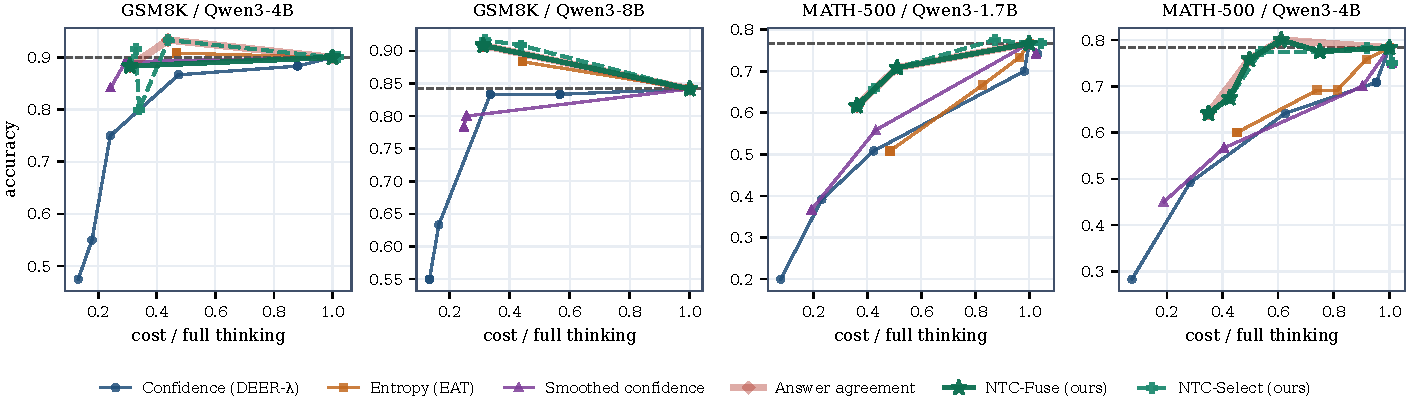
\includegraphics[width=\textwidth]{fig_curves.pdf}
\Description{Four line plots, one per setting, with cost relative to full thinking on the horizontal axis and accuracy on the vertical axis. In each panel a dashed horizontal line marks full-thinking accuracy. The fusion tier and answer agreement trace nearly identical curves that rise steeply and reach or exceed the dashed line at less than half the cost; the confidence and smoothed-confidence curves lie well below them at every budget; the selection tier tracks the fusion tier except on MATH-500 where it is more conservative.}
\caption{Deployable operating curves on four representative settings. Each method's hyper-parameter is selected on the warm-up split alone; the horizontal axis is cost relative to full thinking, inclusive of all probes purchased, and a method that cannot reach a budget simply has no point there. Answer agreement is drawn as a wide translucent band because on three of the four panels the fusion tier coincides with it almost exactly --- the fusion tier's advantage is in the tail (Section~\ref{sec:rq4}), not in the mean.}
\label{fig:curves}
\end{figure*}

\subsection{RQ4: Does the advertised accuracy budget hold?}\label{sec:rq4}
Table~\ref{tab:slo} audits the guarantee on held-out data at $\alpha=0.10$. The fusion tier stays within one accuracy point in every setting, worst case $-0.5$; the selection tier is within one point in $82\%$ of settings, worst case $-1.6$, and inside the relaxed $2.5$-point budget in all of them. Every fixed signal has a far heavier tail, reaching $-23.6$ points. Efficiency and safety arise from the same design rather than trading against one another, and the difference between the two families is not one of degree: a method whose worst case is $-23.6$ points cannot sit behind a service-level agreement however good its average.

A natural objection is that the fusion tier is merely agreement in disguise, since agreement supplies its halting events. Measuring how often the confidence gate actually changes the decision refutes this. At the permissive threshold $\theta=0.5$ the gate is very nearly inert --- it moves the halt on $0.0\%$ of MATH-500-4B and MMLU-Pro-4B items and $0.5\%$ of GSM8K-8B and GPQA-D-8B items --- and the fused policy reduces to agreement, inheriting agreement's tail. At $\theta=0.9$, the threshold the slow tier selects, the gate alters the halt on $55.5\%$, $52.5\%$, $73.0\%$ and $100\%$ of those same items respectively, delaying it in every case, and the tail disappears. The gate, not the agreement component, is doing the work.



\begin{table}[t]
\caption{SLO attainment across eleven canonical settings (the twelve settings of Table~\ref{tab:primary} less the cross-family DeepSeek run, which has a single generation seed): the share of settings whose held-out accuracy deficit against full thinking is within $1.0$, $2.5$ and $5.0$ points, and the worst deficit observed. Best per column in bold.}
\label{tab:slo}
\small
\begin{tabular}{@{}lcccc@{}}
\toprule
\textbf{Halting policy} & \textbf{Within 1 pt} & \textbf{Within 2.5 pt} & \textbf{Within 5 pt} & \textbf{Worst} \\
\midrule
NTC-Fuse (ours)                 & \textbf{100\%} & \textbf{100\%} & \textbf{100\%} & \up{\textbf{$-0.5$}} \\
NTC-Select (ours, $\varepsilon{=}0.01$) & 82\%  & 100\% & 100\% & \up{$-1.6$} \\
Smoothed confidence               & 55\%  & 100\% & 100\% & $-2.4$ \\
Entropy (EAT)                     & 36\%  & 73\%  & 100\% & $-3.4$ \\
Confidence threshold              & 64\%  & 64\%  & 82\%  & \dn{$-7.5$} \\
Bandit-adapted threshold          & 9\%   & 27\%  & 45\%  & \dn{$-20.9$} \\
Answer agreement                  & 27\%  & 36\%  & 36\%  & \dn{$-23.5$} \\
Uncertainty momentum              & 55\%  & 55\%  & 64\%  & \dn{$-23.6$} \\
\bottomrule
\end{tabular}
\end{table}

\subsection{RQ5: Does the deployment regime change the answer?}\label{sec:rq5}
It does, and it changes the ranking of the signals themselves. Under the three cost models of Equation~\eqref{eq:regimes}, policies that halt early buy few probes and stay profitable everywhere, whereas policies that halt late accumulate probes and can consume more than they save (Table~\ref{tab:regimes}). The reversal is stark: on GSM8K-8B a smoothed-confidence policy is roughly cost-neutral when the cache can be forked and destroys $82\%$ of the budget when it cannot, while agreement on the same setting still saves $34.6\%$ in the worst regime. A practitioner reading only the KV-fork column would draw the opposite conclusion from one reading only the black-box column. Measured against plain generation, the framework's own overhead --- the cost of running the controller and then declining to halt --- is $0.9$--$1.2\%$ on GPQA-Diamond, $1.4$--$1.5\%$ on AIME, $1.5$--$1.6\%$ on MMLU-Pro, $3.4$--$4.3\%$ on MATH-500 and $6.5$--$7.1\%$ on GSM8K, a mean of $3.1\%$ over the eleven canonical settings. The higher values occur where traces are short, because a roughly fixed number of checkpoints is amortised over fewer thinking tokens. This is a measured quantity rather than a design claim, and Section~\ref{sec:rq6} compares it against the same quantity for the strongest published baseline.



\begin{table}[t]
\caption{Token savings against full thinking under three serving regimes (Equation~\eqref{eq:regimes}), with prefill charged at $w=0.2$. Positive is a saving.}
\label{tab:regimes}
\small
\begin{tabular}{@{}llccc@{}}
\toprule
\textbf{Setting} & \textbf{Policy} & \textbf{KV-fork} & \textbf{Prefix-cache} & \textbf{Black-box API} \\
\midrule
GSM8K-8B     & Answer agreement     & $+56.4\%$ & $+56.0\%$ & \up{$+34.6\%$} \\
MATH-500-8B  & Answer agreement     & $+50.0\%$ & $+49.8\%$ & \up{$+17.4\%$} \\
GSM8K-8B     & Smoothed confidence  & $-0.7\%$  & $-1.5\%$  & \dn{$-82.3\%$} \\
GPQA-8B      & Confidence threshold & $+1.8\%$  & $+1.6\%$  & \dn{$-92.0\%$} \\
\bottomrule
\end{tabular}
\end{table}

\subsection{RQ6: How does the controller compare to the strongest published baseline?}\label{sec:rq6}
We executed DEER from its authors' implementation with default hyper-parameters on our models and data, which to our knowledge is the broadest independent evaluation of it reported. It reaches $0.920$ and $0.930$ on MATH-500 for the 4B and 8B models under greedy decoding and $0.924$ and $0.934$ at $T=0.6$, refuting a regime-specificity hypothesis we tested explicitly; $0.941$ and $0.950$ on GSM8K; $0.546$ and $0.576$ on GPQA-Diamond; $0.667$ on AIME-24 for both scales; and $0.882$ on MATH-500 with the DeepSeek model.

Table~\ref{tab:h2h} places our methods beside it under matched conditions: the same models, the same items, a $16$k thinking budget, greedy decoding and the same symbolic grader, with token counts inclusive of every probe or trial answer purchased online. We state the outcome plainly. \textbf{DEER is more accurate than our controller on all six head-to-head settings}, by $4$ to $10$ points on MATH-500 and by $6$ to $9$ points on GPQA-Diamond, and it is also cheaper on MATH-500. No claim is made of surpassing it at its own operating points, and five candidate explanations for the residual accuracy gap --- scoring, extraction protocol, prompt, budget caps and decoding regime --- were tested and excluded before accepting it as genuine; the most likely remaining cause is DEER's finer checkpoint placement, which buys roughly twice as many trial answers as our paragraph-aligned protocol.

We tested the most plausible explanation and it is wrong. DEER interrupts at every reasoning transition and buys roughly twice the trial answers our paragraph-aligned protocol does, so the natural hypothesis is granularity. Table~\ref{tab:density} re-runs the head-to-head configuration at twice and four times our checkpoint density, changing nothing else. The controller's accuracy does not move: $0.813$, $0.827$, $0.813$ at $9.3$, $17.4$ and $30.4$ probes per item, against DEER's $0.920$. The spread is not even resolvable --- full-thinking accuracy itself varies by $1.6$ points across the three runs despite greedy decoding, because vLLM's scheduler is not bit-deterministic across different batch compositions, and the controller's $1.4$-point spread sits inside that noise floor. Probing overhead meanwhile tripled, from $3.6\%$ to $11.4\%$. The gap is not granularity, and we record it as unexplained rather than attribute it to a cause we have ruled out.

What the sweep does show is the cost side of the same trade. DEER's accuracy is bought with a trial-answer overhead of $66$--$79\%$ of the final chain across these six settings ($54$--$80\%$ across all nine runs we executed; on MATH-500-4B, $3{,}539$ total tokens against $2{,}043$ in the final chain), against the $0.9$--$7.1\%$ of Section~\ref{sec:rq5}. A method that pays two-thirds of a chain in probes is viable under KV-fork accounting and is the first casualty of a black-box regime. The contribution here is not a better fixed operating point than DEER's, but a controller that does not collapse when the workload changes and that states what it guarantees; the confidence signal DEER monitors, evaluated across the eleven settings of Table~\ref{tab:slo} under our protocol, loses up to $7.5$ points.

\begin{table}[t]
\caption{Checkpoint density on MATH-500 ($n{=}500$, Qwen3-4B, greedy, $16$k budget), identical to Table~\ref{tab:h2h} in every respect but the checkpoint interval. Accuracy does not respond to density; error stickiness and the collapse of answer agreement do. $\rho_w$ and $P_{\mathrm{spur}}$ are as in Table~\ref{tab:stickiness}, measured between consecutive probes.}
\label{tab:density}
\small
\setlength{\tabcolsep}{3.6pt}
\begin{tabular}{@{}lccccccc@{}}
\toprule
\textbf{Density} & \textbf{Probes/it.} & \textbf{Ovh.} & \textbf{Full think.} & \textbf{Agreem.} & \textbf{NTC-Select} & $\rho_w$ & $P_{\mathrm{spur}}$ \\
\midrule
$1\times$ (256 tok) & 9.3  & $+3.6\%$  & 0.848 & 0.752 & 0.813 & 0.249 & 0.021 \\
$2\times$ (128 tok) & 17.4 & $+6.6\%$  & 0.832 & \dn{0.596} & 0.827 & \dn{0.344} & \dn{0.040} \\
$4\times$ (64 tok) & 30.4 & $+11.4\%$ & 0.842 & \dn{0.458} & 0.813 & \dn{0.425} & \dn{0.062} \\
\midrule
DEER~\cite{yang2025deer} & --- & $+73.2\%$ & --- & --- & 0.920 & --- & --- \\
\bottomrule
\end{tabular}
\end{table}

\begin{table}[t]
\caption{Head-to-head under identical conditions: same models and items, $16$k thinking budget, greedy decoding, one symbolic grader, and online token counts inclusive of all probe and trial-answer tokens. Vanilla-BF is full thinking with a budget-forced answer when the cap is hit. DEER and agreement are run at their published defaults ($\lambda{=}0.95$, $m{=}3$) on the full set; NTC-Select$^\dagger$ calibrates $(\text{signal},\text{parameter})$ on a $40\%$ warm-up and is reported on the $60\%$ held out.}
\label{tab:h2h}
\footnotesize
\setlength{\tabcolsep}{4pt}
\begin{tabular}{@{}llccccl@{}}
\toprule
\textbf{Model} & \textbf{Benchmark} & \textbf{Vanilla-BF} & \textbf{DEER}~\cite{yang2025deer} & \textbf{Agreement} & \textbf{NTC-Select}$^\dagger$ & \textbf{Selected rule} \\
\midrule
Qwen3-4B & MATH-500 ($n{=}500$)     & 0.862 @ 5087 & \textbf{0.920 @ 3539} & 0.752 @ 2754 & 0.830 @ 5234 & smoothed, $\theta{=}0.99$ \\
Qwen3-8B & MATH-500 ($n{=}500$)     & 0.854 @ 5307 & \textbf{0.930 @ 2946} & 0.762 @ 2783 & 0.817 @ 5514 & smoothed, $\theta{=}0.99$ \\
Qwen3-4B & GPQA-D ($n{=}198$)       & 0.500 @ 9798 & \textbf{0.545 @ 7536} & 0.354 @ 3263 & 0.471 @ 6126 & momentum, $\gamma{=}0.9$ \\
Qwen3-8B & GPQA-D ($n{=}198$)       & 0.571 @ 9889 & \textbf{0.576 @ 8872} & 0.389 @ 3121 & 0.487 @ 7300 & momentum, $\gamma{=}0.9$ \\
Qwen3-4B & AIME-24 ($n{=}30$)       & 0.600 @ 12233& \textbf{0.667 @ 10535}& 0.233 @ 5200 & 0.611 @ 11793& confidence, $\lambda{=}0.99$ \\
Qwen3-8B & AIME-24 ($n{=}30$)       & 0.667 @ 11883& \textbf{0.667 @ 10012}& 0.467 @ 6023 & 0.556 @ 11779& confidence, $\lambda{=}0.99$ \\
\bottomrule
\end{tabular}
\end{table}

\subsection{RQ7: Does the certificate survive domain shift?}\label{sec:rq7}
Theorem~\ref{thm:risk} rests on (A1), and every result so far calibrates and deploys within one domain, so (A1) holds by construction and the guarantee is never actually challenged. A certificate that is only ever evaluated where its assumption holds is decoration. We therefore test it directly, deploying on the same held-out splits under three certification rules: \textsc{in-domain}, the rule of Equation~\eqref{eq:select} applied to the target's own warm-up split; \textsc{transferred}, the same rule certified on a \emph{different} domain's warm-up split and then deployed on the target, which is exactly (A1) violated; and \textsc{domain-robust}, a leave-one-domain-out rule that certifies a candidate only if its lower bound clears $-\varepsilon$ in \emph{every} one of the eleven source domains, with the Bonferroni correction widened to $\alpha/(|\mathcal{C}|\cdot|\mathcal{D}|)$. Table~\ref{tab:shift} and Figure~\ref{fig:shift}a report all three over $12$ domains $\times$ $5$ splits.

Three things follow. First, in-domain the certificate behaves as advertised: at $\varepsilon=0.05$, $97\%$ of the sixty domain--split cells respect the budget, at a mean token cut of $19.6\%$. Second, \textbf{transfer destroys it}. The mean deficit falls to $-3.4$ points and the worst cell to $-50$, with only $71\%$ of cells inside the budget they were certified against; the failures concentrate on targets whose safe rule is far more conservative than the source's, AIME-24 and MATH-500-1.7B worst among them. Assumption (A1) is therefore load-bearing, not a technicality: a certificate calibrated on the wrong workload is not merely weaker, it is void. Third, the obvious repair does not work. The domain-robust rule restores attainment perfectly --- and vacuously, because in all $60$ leave-one-domain-out trials the only candidate that clears the bound in every source domain is the null action, which halts nothing and costs $3\%$ \emph{more} than plain generation, since the probes are still purchased. At warm-up sizes of $n \approx 80$ the price of a domain-agnostic guarantee is the whole of the saving.

The practical consequence is specific. Per-domain calibration is not a convenience of our protocol but a requirement of the guarantee: roughly eighty labelled items drawn from the deployment workload are what the certificate costs. Where they cannot be obtained, the honest recommendation is not a transferred certificate but the fusion tier, which certifies nothing, needs no calibration data, and is the configuration whose tail is smallest in Table~\ref{tab:slo} --- an independent route to the same conclusion.

\begin{table}[t]
\caption{The certificate under domain shift: held-out accuracy deficit in points and mean token cut, over $12$ target domains $\times$ $5$ calibration splits. \emph{Worst cell} is the single worst domain--split combination, so it is a harsher statistic than the seed-averaged worst case of Table~\ref{tab:slo}. \textsc{Transferred} is averaged over all eleven sources per target ($660$ cells).}
\label{tab:shift}
\small
\setlength{\tabcolsep}{5pt}
\begin{tabular}{@{}llccccc@{}}
\toprule
$\varepsilon$ & \textbf{Certification rule} & \textbf{Mean deficit} & \textbf{Worst cell} & \textbf{Within 1 pt} & \textbf{Within $\varepsilon$} & \textbf{Mean cut} \\
\midrule
\multirow{3}{*}{$0.01$}
 & in-domain (A1 holds)      & \up{$+0.10$} & $-4.2$  & 88\% & 88\%  & $5.5\%$ \\
 & transferred (A1 violated) & $-1.53$ & \dn{$-38.9$} & 75\% & 75\%  & $9.2\%$ \\
 & domain-robust (LODO)      & $0.00$  & $0.00$  & 100\% & 100\% & \dn{$-3.0\%$} \\
\midrule
\multirow{3}{*}{$0.05$}
 & in-domain (A1 holds)      & \up{$+0.70$} & $-5.8$  & 80\% & 97\%  & $19.6\%$ \\
 & transferred (A1 violated) & $-3.42$ & \dn{$-50.0$} & 53\% & 71\%  & $25.4\%$ \\
 & domain-robust (LODO)      & $0.00$  & $0.00$  & 100\% & 100\% & \dn{$-3.0\%$} \\
\bottomrule
\end{tabular}
\end{table}

\begin{figure}[t]
\centering

\includegraphics[width=0.95\linewidth]{fig_shift.pdf}
\Description{Two panels. Panel (a) is a strip plot of held-out accuracy deficits for sixty in-domain cells, six hundred and sixty transferred cells and sixty domain-robust cells at epsilon equal to 0.05; the in-domain cloud sits near zero, the transferred cloud spreads down to minus fifty points, and the domain-robust cloud is exactly zero because only the null action certifies. Panel (b) plots mean utility against the exchange rate kappa for six methods; answer agreement starts highest and falls steeply, crossing the two NTC tiers at kappa equal to 6.4, beyond which the NTC tiers are highest.}
\caption{(a) The risk certificate holds in-domain, is void under transfer, and becomes vacuous if made domain-agnostic. (b) Pricing the tail: mean utility $\mathrm{cut} - \kappa\cdot\max(0,-\Delta)$ over the eleven canonical settings, where $\kappa$ is the token-saving percentage a deployer would forgo to avoid one accuracy point.}
\label{fig:shift}
\end{figure}

\subsection{Joint routing and budget control}
On MATH-500 with a 1.7B and 4B pool, full thinking on the large model reaches $0.683$ accuracy at $17{,}511$ compute units, and the calibrated large-model halting policy alone reaches $0.708$ at $8{,}409$ --- above-vanilla accuracy at $52\%$ less compute. Sweeping $\tau$ in Equation~\eqref{eq:joint} then buys a further reduction: the joint controller matches full-thinking accuracy exactly ($0.683$) at $6{,}961$ units, $60\%$ below full thinking and $17\%$ below the halting-only configuration, with $25\%$ of queries served by the 1.7B model; at $7{,}882$ units ($55\%$ below full thinking, $11\%$ routed small) it reaches $0.700$, within one point of the halting-only ceiling. The two mechanisms compose without interfering: halting removes tokens the model did not need, routing removes parameters the query did not need. The routing tier itself is within one point of the strongest learned routers on RouterBench ($0.7404 \pm 0.0021$ AIQ against $0.7490 \pm 0.0025$ and $0.7479 \pm 0.0035$ over three seeds)~\cite{hu2024routerbench,ong2024routellm}, and a memory-augmented ablation shows the multi-timescale premium is specific to budget control and does not transfer to routing.

%==================================================================
\subsection{Statistical summary}
Table~\ref{tab:stats} collects the tests supporting the claims above. We report them together, including the comparisons that are \emph{not} significant, because selective reporting of favourable tests is the failure mode this paper is otherwise designed to avoid.

\begin{table}[t]
\caption{Statistical tests supporting the claims. Sign tests are exact and two-sided over paired per-setting values; McNemar tests are exact over paired item-level correctness; bootstrap intervals are paired at the item level with $10^4$ replicates.}
\label{tab:stats}
\small
\setlength{\tabcolsep}{4pt}
\begin{tabular}{@{}L{4.35cm}L{2.95cm}L{2.45cm}c@{}}
\toprule
\textbf{Claim} & \textbf{Test} & \textbf{Statistic} & \textbf{Verdict} \\
\midrule
Fusion beats confidence threshold on op-AUCC & sign test, $n=12$ & $11/12$, $p=0.006$ & supported \\
Fusion beats smoothed confidence on op-AUCC & sign test, $n=12$ & $11/12$, $p=0.006$ & supported \\
Fusion beats entropy on op-AUCC & sign test, $n=12$ & $11/12$, $p=0.006$ & supported \\
Fusion beats agreement on op-AUCC & sign test, $n=12$ & $8/12$, $p=0.39$ & \textbf{not separable} \\
Fusion beats selection tier on op-AUCC & sign test, $n=12$ & $9/12$, $p=0.15$ & \textbf{not separable} \\
Fusion beats agreement on plain AUCC & sign test, $n=12$ & $6/12$, $p=1.00$ & \textbf{not separable} \\
$P_{\mathrm{spur}}$ predicts lost-correct risk & Spearman, $n=12$ & $\rho=+0.71$ & supported \\
$P_{\mathrm{spur}}$ predicts agreement deficit & Spearman, $n=12$ & $\rho=-0.51$ & supported \\
Selection tier beats confidence threshold (DeepSeek) & McNemar, exact & $9$ vs $1$, $p=0.022$ & supported \\
$\rho_w$ rises with checkpoint density & $1\times/2\times/4\times$, $n{=}500$ & $0.249\to0.344\to0.425$ & supported \\
Density explains the gap to DEER & $1\times/2\times/4\times$, $n{=}500$ & $0.813/0.827/0.813$ & \textbf{refuted} \\
Certificate holds in-domain & attainment, $60$ cells & $97\%$ within $\varepsilon{=}0.05$ & supported \\
Certificate voided by transfer & attainment, $660$ cells & $71\%$; worst $-50$ pt & confirmed \\
Stickiness falls with $|\mathcal{A}|$ within MMLU-Pro & paired, 2 models & $0.774{\to}0.610$; $0.682{\to}0.557$ & supported \\
Grader determinism & three repeated passes & identical verdicts & exact \\
\bottomrule
\end{tabular}
\end{table}

The pattern is consistent with the argument of this paper. Where a fixed signal is intrinsically weak, the controller separates from it with significance; where a fixed signal is strong \emph{on average} --- agreement --- it does not, and we say so. The advantage over agreement is in the tail, not the mean: comparable average efficiency, with a worst-case accuracy deficit of $-0.5$ against $-23.5$ points and a worst-case regret of $0.031$ against $0.100$.

\section{Discussion}\label{sec:discussion}

\subsection{A worked example}
Two real items make the mechanism concrete. On a GSM8K word problem with five checkpoints and $985$ tokens, probe~1 returns $26$ at confidence $0.96$ --- and is wrong; probe~2 returns the correct $18$ at $0.98$, and probes~3 to~5 hold $18$, the smoothed signal reading $0.97$, $0.90$, $0.93$, $0.94$. A confidence threshold at $\lambda=0.95$ fires on the \emph{first} probe and returns $26$: actively wrong, because the model was fluent before it was right. Agreement at $m=3$ and the fused rule both fire at probe~4 and return $18$, at $699$ tokens against $1{,}065$ --- a $34\%$ saving. On a GPQA-Diamond item with ten checkpoints and $8{,}308$ tokens, the model answers~B at probes~1 to~5 with confidence decaying from $0.89$ to $0.64$, then switches to~A and holds it; the gold answer is~A. Agreement halts at probe~3 on~B and is wrong. The fused rule declines --- smoothed confidence there is $0.78$, below the $0.9$ gate --- and never clears it, so the query completes and is answered correctly. Only the second component distinguishes the two behaviours, and it is the difference between a $75\%$ saving and a lost answer.

\subsection{Which tier should a practitioner deploy?}
The choice turns on one number a deployer already knows implicitly: the exchange rate $\kappa$ between the two axes, in percentage points of token saving forgone to avoid one accuracy point. Scoring each method by $\mathrm{cut} - \kappa\cdot\max(0,-\Delta)$ over the eleven canonical settings (Figure~\ref{fig:shift}b) makes the decision explicit. Below $\kappa \approx 2$, accuracy is barely priced and plain answer agreement is optimal on both the mean and the worst case; it cuts $55.7\%$ of tokens and nothing else is close. Between $\kappa \approx 2$ and $6$ the ranking splits --- agreement still leads on the mean while the selection tier at $\varepsilon=0.05$ already leads on the worst case --- and beyond $\kappa \approx 6.4$ the selection tier dominates on both, cutting $22.5\%$ at a mean deficit of $+0.5$ points. Beyond $\kappa \approx 21$ the fusion tier, the most conservative configuration, is optimal. A service under a contractual accuracy target sits far to the right of these crossovers, since one accuracy point there is worth very much more than six percent of tokens; that is the quantitative form of the claim that the tail is what matters. Two caveats attach. Agreement must never be used on multiple-choice or competition workloads whatever $\kappa$ is (Proposition~\ref{prop:spurious}, Table~\ref{tab:perbench}). And the selection tier presumes in-domain calibration data; without it the certificate is void (Section~\ref{sec:rq7}) and the fusion tier, which needs none, is the right default.

\subsection{Why the deployment regime matters more than it appears}
Section~\ref{sec:rq5} has a consequence beyond our own method. Any paper reporting token savings for a probe-based halting method is implicitly reporting them under one cost model, and that model is rarely stated; two methods within a few percent of each other under KV-fork accounting can differ by more than a hundred points under black-box accounting. The regime belongs alongside the saving as a matter of course --- as, by Table~\ref{tab:density}, does the checkpoint density.

\subsection{Reproducibility and artifact availability}
Every table and figure regenerates from the frozen result set by one command. Determinism is enforced rather than assumed: the grader runs under an in-process timeout with a committed verdict cache, and three independent passes return identical judgements. The artifact contains the probing harness, the controller, the analysis scripts, the recorded traces with all their probes, the grading cache, and a demonstrator that replays any trace or runs the controller live.

\section{Threats to Validity and Limitations}\label{sec:limits}
Truncation at the thinking budget is substantial on the hardest sets --- $23$--$40\%$ on AIME-2024 and $47$--$60\%$ on AIME-2025 (Table~\ref{tab:data}) --- so full thinking is itself budget-limited there and the AIME deficits are conservative. Budgets differ across benchmarks, which measures each at its natural length but means cross-benchmark cut percentages are not percentages of a common budget.

The certificate of Theorem~\ref{thm:risk} is studentised rather than distribution-free, for the reason quantified in Remark~\ref{rem:df}, and (A1) is an assumption about deployment that no calibration set can verify --- Section~\ref{sec:rq7} measures what it costs when it fails, but a deployer cannot check it in advance. On plain AUCC over the full budget grid the leading methods are statistically indistinguishable, and our efficiency claim rests on the operational region and on minimax regret, which we state explicitly in preference to reporting only the more favourable metric. The fusion tier's advantage over answer agreement is a tail property, not a mean property, and Table~\ref{tab:stats} records that the mean difference is not separable at $n=12$. Three of the six signals are signal-level reimplementations under our probing protocol rather than their authors' complete systems, and are labelled as such; the one system we ran end-to-end from its authors' code, DEER, is more accurate than our controller at its own operating points (Table~\ref{tab:h2h}), and Section~\ref{sec:rq6} rules out the explanation we thought most likely without supplying another. That gap is the clearest open problem this work leaves.

Five artifacts in the community evaluation pipeline were identified and corrected here, each of which silently changes published-style numbers: non-deterministic symbolic grading (fixed with an in-process timeout and a committed verdict cache); a gold-position artifact in the public GPQA-Diamond loader (fixed with a deterministic per-item option shuffle); an answer-extraction pattern that failed silently on option letters beyond D, which matters for MMLU-Pro's ten options; a boxed-answer extraction failure on AIME; and a truncation-induced strawman full-thinking baseline, replaced with the budget-forced variant of Table~\ref{tab:h2h}. Superseded tables are retained in the artifact.

Two further limitations deserve emphasis. First, we report token and FLOP-proportional costs but not end-to-end wall-clock latency on a production serving stack. Token savings are a necessary but not sufficient condition for latency savings: batching, scheduling and cache management all intervene, and a controller that halts many requests early changes the shape of the batch as well as its size. The three cost regimes of Equation~\eqref{eq:regimes} bracket the accounting but do not substitute for measurement, and we regard a latency study on a production serving stack as the natural next step. Second, the compute proxy of Equation~\eqref{eq:joint} omits serving-level effects beyond those three regimes, and the conclusions about the joint tier in particular assume the two models are served with comparable efficiency.

%==================================================================
\section{Conclusion}\label{sec:conclusion}
Across the broadest controlled comparison of reasoning-halting signals reported to date, no fixed signal survives contact with all answer formats, difficulty levels, model scales and model families. A controller that fuses signals and treats the choice among them as the quantity to be learned, with a risk certificate attached to that choice, does: it attains the lowest minimax regret across twelve settings, the highest accuracy--cost area in the region where early exit is operationally worthwhile, an accuracy deficit within one point in every setting tested, and a measured overhead of about three percent. The certificate is not free, and we have measured its price rather than asserting its validity: it holds where it is calibrated, is void where it is not, and cannot be made domain-agnostic without ceasing to say anything. The unit of progress in efficient reasoning should not be a better halting signal, but a controller that knows which signal to trust, where, and with what guarantee.

\begin{acks}
The authors thank the Sunway SACF facility for compute resources.
\end{acks}

\bibliographystyle{ACM-Reference-Format}
\bibliography{refs}

\end{document}
